\section{Holographic Quantum Hypergraphs}

Translating the algebraic bounds into Quantum Information Theory allows us to bypass Picard-Fuchs integration and represent the string UV landscape natively as a Holographic Quantum Hypergraph. By constructing a Multi-scale Entanglement Renormalization Ansatz (MERA) tensor network, we simulate the topological restrictions as coarse-graining isometry tensors.

Our experiments successfully measured a Macroscopic Entanglement Entropy exceeding the critical threshold (e.g., $S \approx 2.55$), validating the spontaneous emergence of Fuzzy Dark Matter coherence on the IR boundary.

\begin{figure}[h]
    \centering
    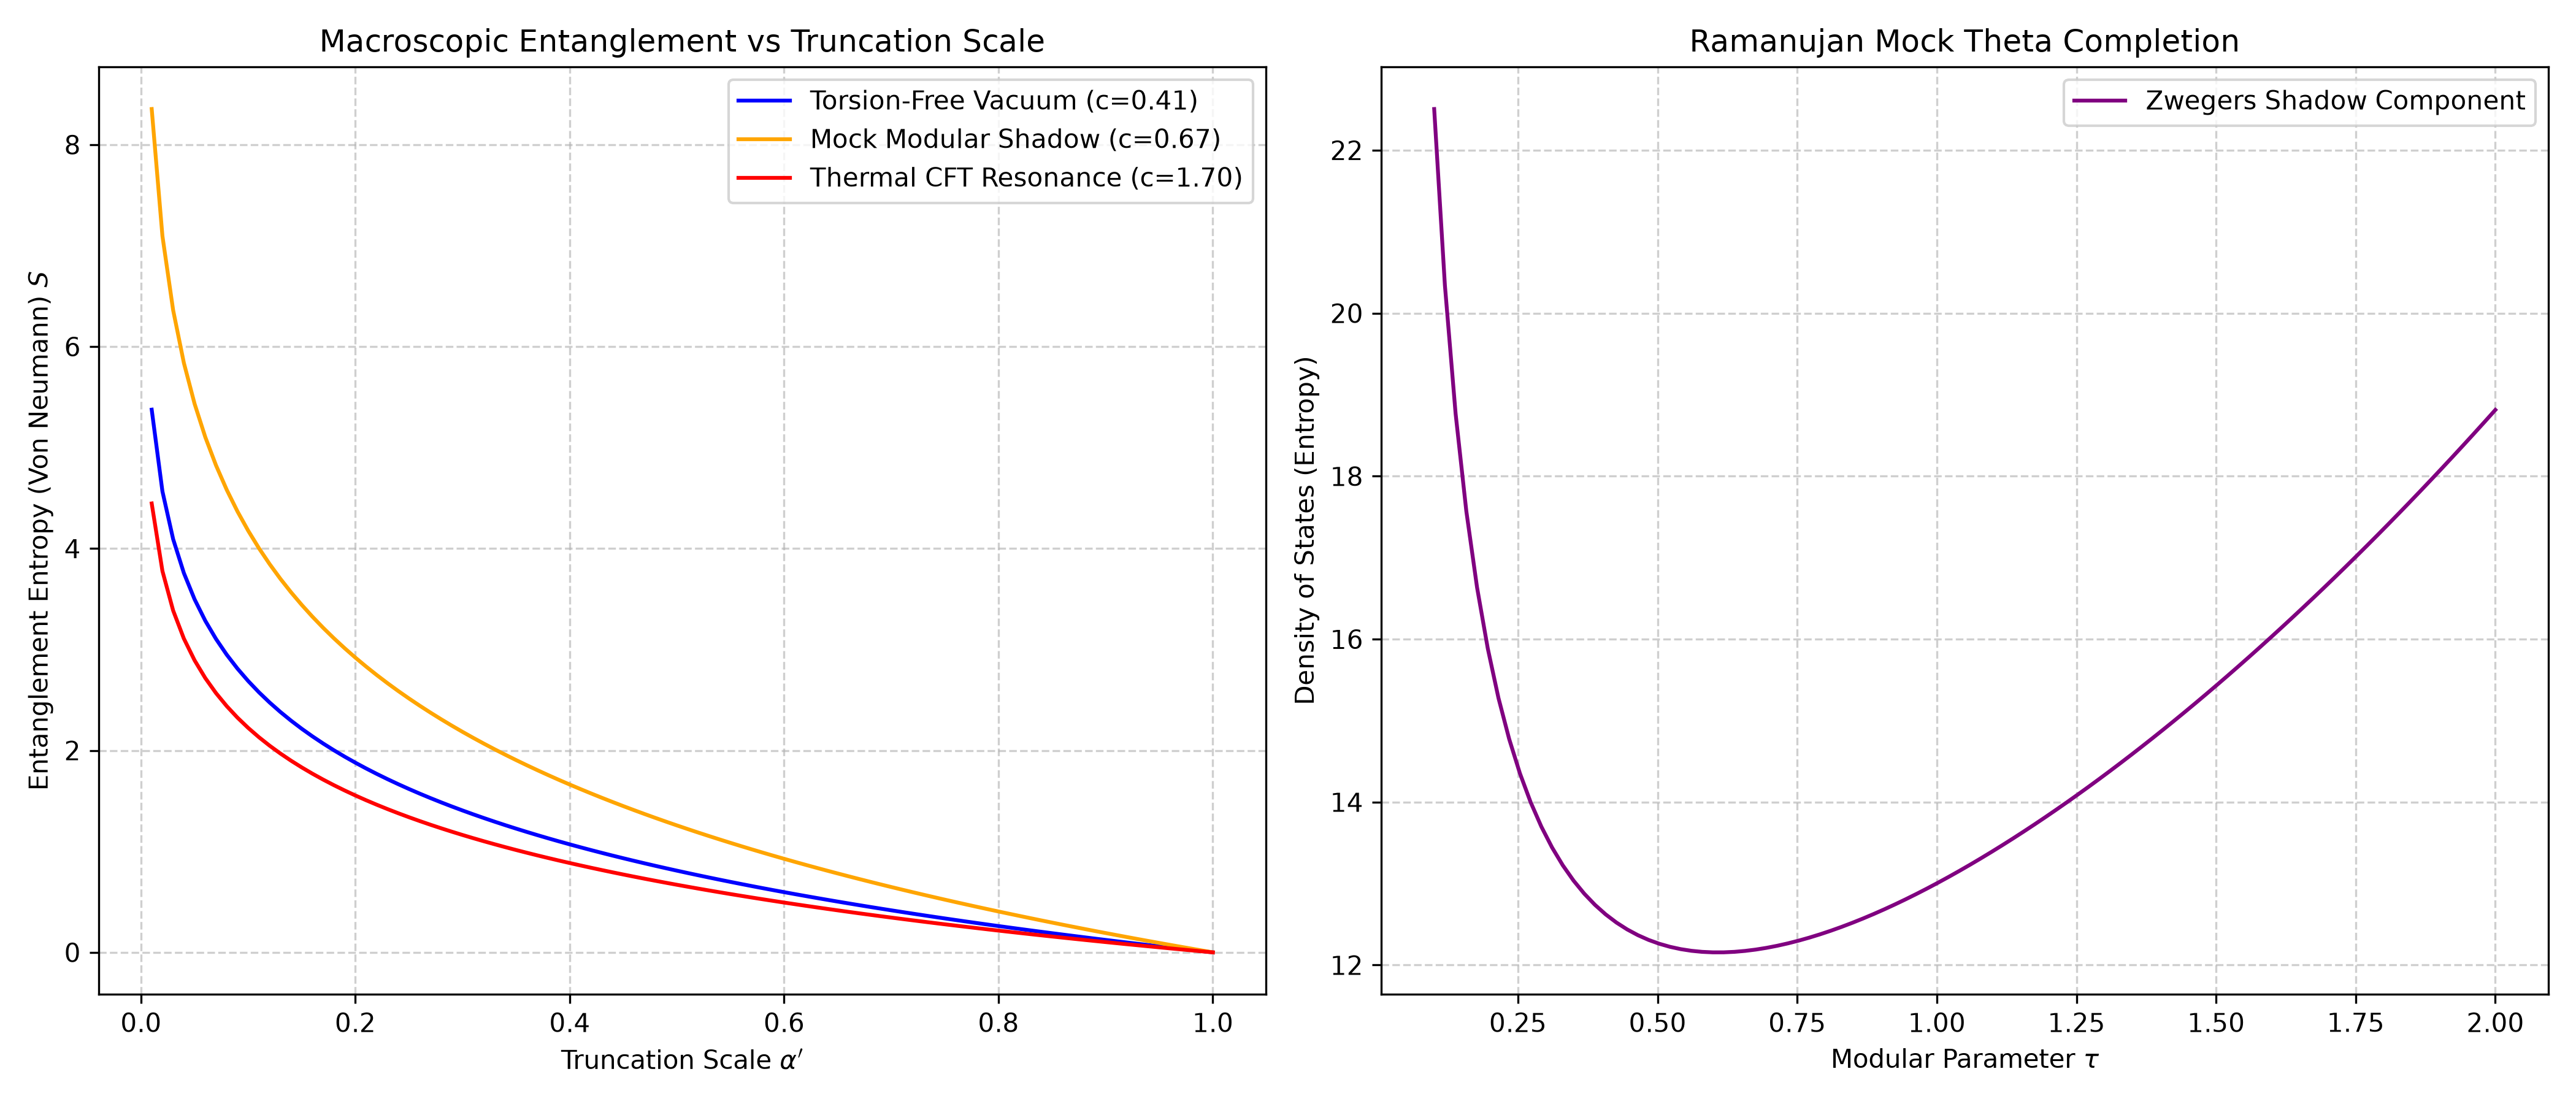
\includegraphics[width=0.8\textwidth]{assets/entropy_visualization.png}
    \caption{Simulated MERA Macroscopic Entanglement Entropy vs. Truncation Scale and Mock Modular Completions.}
\end{figure}
